\chapter[Joint Variable Selection for Omic Biomarkers in Age-at-Diagnosis Data][Joint Variable Selection for Omic Biomarkers]{Joint Variable Selection for Omic Biomarkers in Age-at-Diagnosis Data}
\label{ch:vampw}

\section{Introduction}
\label{sec:intro}
Aging is the primary risk factor for the vast majority of common chronic, noncommunicable diseases that cause illness and death worldwide. The relationship is generally exponential, where disease risk and incidence increase sharply with advancing age~\cite{Kopp2024-hy}. The potential genes and pathways involved in disease onset and progression can be identified by associating time-to-diagnosis information contained within electronic health records to multiple genomic (``multiomics") measures~\cite{gadd_blood_2024, sun_plasma_2023}. The prognostic biomarkers identified can then provide predictors of age at disease onset, facilitating patient screening programs and preventative medicine~\cite{gadd_blood_2024, sun_plasma_2023}.

To date, the two main tasks in time-to-event modeling of multiomics data---association testing and out-of-sample prediction of disease onset age---are almost always conducted using semiparametric \acrfull{coxph} models. More precisely, association testing of disease onset age in genomic studies has predominantly been conducted with marginal CoxPH testing~\cite{gadd_blood_2024,gong_unraveling_2025,deng_atlas_2025}. This corresponds to analyzing one genomic feature at a time, and it ignores pervasive correlations among genomic measures~\cite{argentieri_proteomic_2024}, making it difficult to identify which proteins are most likely driving the observed patterns, with an increased risk of false discoveries \cite{fan_stable_2024}. For prediction tasks, penalized CoxPH models \cite{tibshirani_lasso_1997} are frequently employed \cite{gadd_blood_2024,kuo_proteomic_2025}, enabling the simultaneous modeling of many markers while shrinking or zeroing out a subset of coefficients. Cross-validation is commonly used to select the optimal level of penalization and stability selection \cite{meinshausen_stability_2010} can further be applied to reduce the impact of stochastic variability in model fitting when identifying associated predictors. In practice, this involves fitting multiple models with fixed hyperparameters and selecting only stable features—those that are included in a significant proportion of the models. The CoxPH model relies on a partial likelihood that ignores the baseline hazard and the exact spacing between events. While this makes semi-parametric Cox regression robust and widely applicable, it is statistically less efficient because it depends only on the ordering of event times rather than their absolute values. Hence, it does not provide direct predictions of absolute event times. Instead, it yields relative risk scores with respect to other individuals in the dataset. 

Here, we provide an alternative %address the limitations of semi-parametric models and the false discoveries of marginal testing 
to semi-parametric models by introducing vampW, a joint estimation procedure based on \acrfull{vamp} \cite{rangan_vector_2019,schniter_vector_2016} that employs a fully parametric Weibull survival model. The methodological novelty of vampW lies in the introduction of Weibull channel denoisers and in handling right-censoring. Using large-scale proteomics data linked to electronic health records~\cite{sun_plasma_2023,hu_proteome-wide_2025,wang_blood_2025}, we conduct extensive simulations and benchmarking analyses to demonstrate that joint modeling of time-to-event outcomes using vampW substantially reduces false-positive protein associations, as compared to conventional one-protein-at-a-time testing and other forms of CoxPH models. Applying vampW to 24 disease outcomes in the \acrlong{ukb}, we identify 1,308 and 219 protein-disease associations in models with and without exponential age correction, respectively, highlighting the sensitivity of protein-outcome associations to the choice of age-correction method. In addition to identifying several well-established biomarkers, such as \emph{APOE} with Alzheimer, \emph{REN} with hypertension and \emph{KLK3} with prostate cancer, we find novel associations that may point to previously unrecognized disease pathways. In particular, we identify \emph{CXCL17}, previously reported as a potential biomarker for colorectal cancer and ischemic heart disease, as being associated with depression. The majority of vampW findings replicate in an independent Icelandic cohort, when adjusted for overlap in proteins and outcomes, despite different measurement technologies between the studies. Moreover, across 14 outcomes with sufficient prevalence for out-of-sample evaluation, vampW predicts age at onset with an average root mean squared error which is over 32\% and 26\% lower than that of CoxPH variants and the deep learning approach DeepSurv \cite{katzman_deepsurv_2018}, respectively. We then show that the \acrfull{prs} generated by vampW are transferable across diverse genetic ancestries, even in minority populations. Finally, we show that vampW outperforms deep learning methods in the data-scarce regimes on standard survival benchmarking datasets, demonstrating the utility of our approach across datasets in the life sciences.

\section{Results}
\label{sec:results}

\subsection{Overview of the approach}
Our aim is to jointly model the data in a design matrix $\bm{X} \in \mathbb{R}^{N \times P}$, containing observations on $N$ individuals and $P$ biological markers, ensuring that we control for the correlation structure. 
%Our goal is to jointly model $N$ individuals and $P$ biological markers within the design matrix $\bm{X} \in \mathbb{R}^{N \times P}$, ensuring that we control for correlation structure. 
We consider a Weibull model for time-to-event observations, $\mathbf{y} = [y_1, \dots, y_N]^\top$, where $y_i$ denotes the time-to-event (diagnosis) for individual $i$. The model is formulated as follows:
% Using the fact that the mean and variance can be separated in the Weibull model and that the logarithm of a Weibull random variable follows a Gumbel distribution, we formulate the model as:
\begin{equation}
    \label{eq:vampW_model_overview}
    \log (\bm{y} )=\mu + \bm{X} \bm{\beta} + \frac{\bm{w}}{\alpha} + \frac{K}{\alpha}, 
\end{equation}
where $\bm{w} = [w_1, \dots, w_N]$ is a random vector containing independent, Gumbel$(0,1)$ distributed variables, $\alpha$ is the Weibull shape parameter, $\bm{\beta}$ is the vector of marker effects, $\mu$ is the model intercept, and $K$ is the Euler-Mascheroni constant. We normalize the entries of $\bm{X}$ to have zero mean and unit variance across columns. In order to allow for a range of effect magnitudes, we select the prior on $\bm{\beta}$ to be an adaptive spike-and-slab form:
\begin{equation}
\label{eq:prior_overview}
    \beta_j \sim ( 1 - \lambda ) \delta_0 + \lambda \sum^L_{i=1} \pi_i \cdot \mathcal{N}(0, \sigma^2_i),
\end{equation}
where $L$ denotes the number of mixture components, $(\pi_1, \dots, \pi_L)$ are inclusion probabilities, $(\sigma^2_1, \dots, \sigma^2_L)$ are mixture-specific variances, $\delta_0$ is a Dirac spike function at 0, and $\lambda$ is the sparsity rate (for full details see Methods).

To fit the parameters of the model outlined in Equation~\eqref{eq:vampW_model_overview}, we introduce a novel generalized vector approximate message passing algorithm (called \emph{vampW}), %employing a  framework \cite{rangan_vector_2019,schniter_vector_2016}, 
which adaptively estimates the prior-specific parameters from Equation \eqref{eq:prior_overview} and Weibull distribution parameters of Equation~\ref{eq:vampW_model_overview} via an \acrfull{em} procedure. %Approximate message passing (AMP) \cite{DMM09,feng2022unifying} refers to a family of iterative algorithms with several attractive properties for the proposed application, namely \emph{(i)} allowing the use of a wide range of Bayesian priors, \emph{(ii)} achieving Bayes-optimal performance in several settings \cite{barbier-mmse-glm-pnas,montanari2017estimation,mondelli2021approximate,barbier2023fundamental}, and \emph{(iii)} enabling association test statistics to be obtained via state evolution \cite{Bayati2011,bolthausen2014iterative}, a low-dimensional recursion tracking the probability distributions of objects inside the algorithm. 
A recent study \cite{Depope2026} has demonstrated that a vector approximate message passing framework can be applied to imputed and whole-genome sequence data to achieve state-of-the art polygenic risk score performance for human complex traits.
% the authors demonstrated the applicability of the AMP framework to genome-wide association studies (GWAS) and whole genome sequence data (WGS). 
%However, the model considered by \cite{Depope2026} is linear and the data considered is not censored.
% , as is standard in GWAS and WGS. 
Here, we develop this framework further for age-at-onset phenotypes, where the majority of the data is right-censored. The Weibull model we employ, whose applicability to omics and medical data is well documented in the literature~\cite{Ojavee2021-zu, plana_cancer_2022,duan_bayesian_2018}, is highly non-linear and we: \textit{(i)} introduce a novel Weibull channel denoiser, and \textit{(ii)} a novel method for handling right-censored data. % within the VAMP framework. 
These properties make vampW broadly applicable to biological datasets integrated with electronic medical records containing information on disease onset times.

%in contrast, we analyze protein abundance measurements from the UK Biobank Pharma Proteomics Project (PPP) dataset \cite{sun_plasma_2023} paired with age-at-onset phenotypes, where the majority of the data is right-censored, see Section \ref{subsec:W} for details. Furthermore, 
% These properties make vampW broadly applicable to biological datasets linked to medical records for predicting the time to disease onset.
% enabling the joint modeling of time-to-onset of human complex diseases.
Within a single framework, vampW performs variable selection using \acrlongpl{pip} (PIPs, see Methods), while simultaneously enabling time-to-event prediction. Here, we apply this model to analyze protein abundance measurements from the \acrfull{ukb_ppp} dataset \cite{sun_plasma_2023} paired with age-at-onset phenotypes. As compared to the marginal CoxPH testing that has previously been used for these data~\cite{gadd_blood_2024,gong_unraveling_2025,deng_atlas_2025}, the key differences are that within vampW: \textit{(i)} all proteins are modeled jointly, capturing combined effects and controlling for correlations among plasma protein abundances; \textit{(ii)} an interpretable hazard structure is used where depending on the value of its shape parameter, the hazard rate can increase, decrease, or remain constant over time; \textit{(iii)} a full-likelihood exploits the actual event times directly, capturing the probability of the observed data under the complete model specification; \textit{(iv)} a continuous survival curve can generate long-term survival predictions because its parametric form is defined over the full time domain, whereas the Cox model paired with the Breslow estimator yields a piecewise-defined baseline hazard; and \textit{(v)} prior knowledge or specific information can be incorporated within the Bayesian framework and posterior mean estimates are produced together with credible intervals, allowing for explicit quantification of uncertainty.


\subsection{Simulation study in UKB PPP}
\label{sim_ukb_ppp}

\begin{figure}[t]
    \begin{center}
    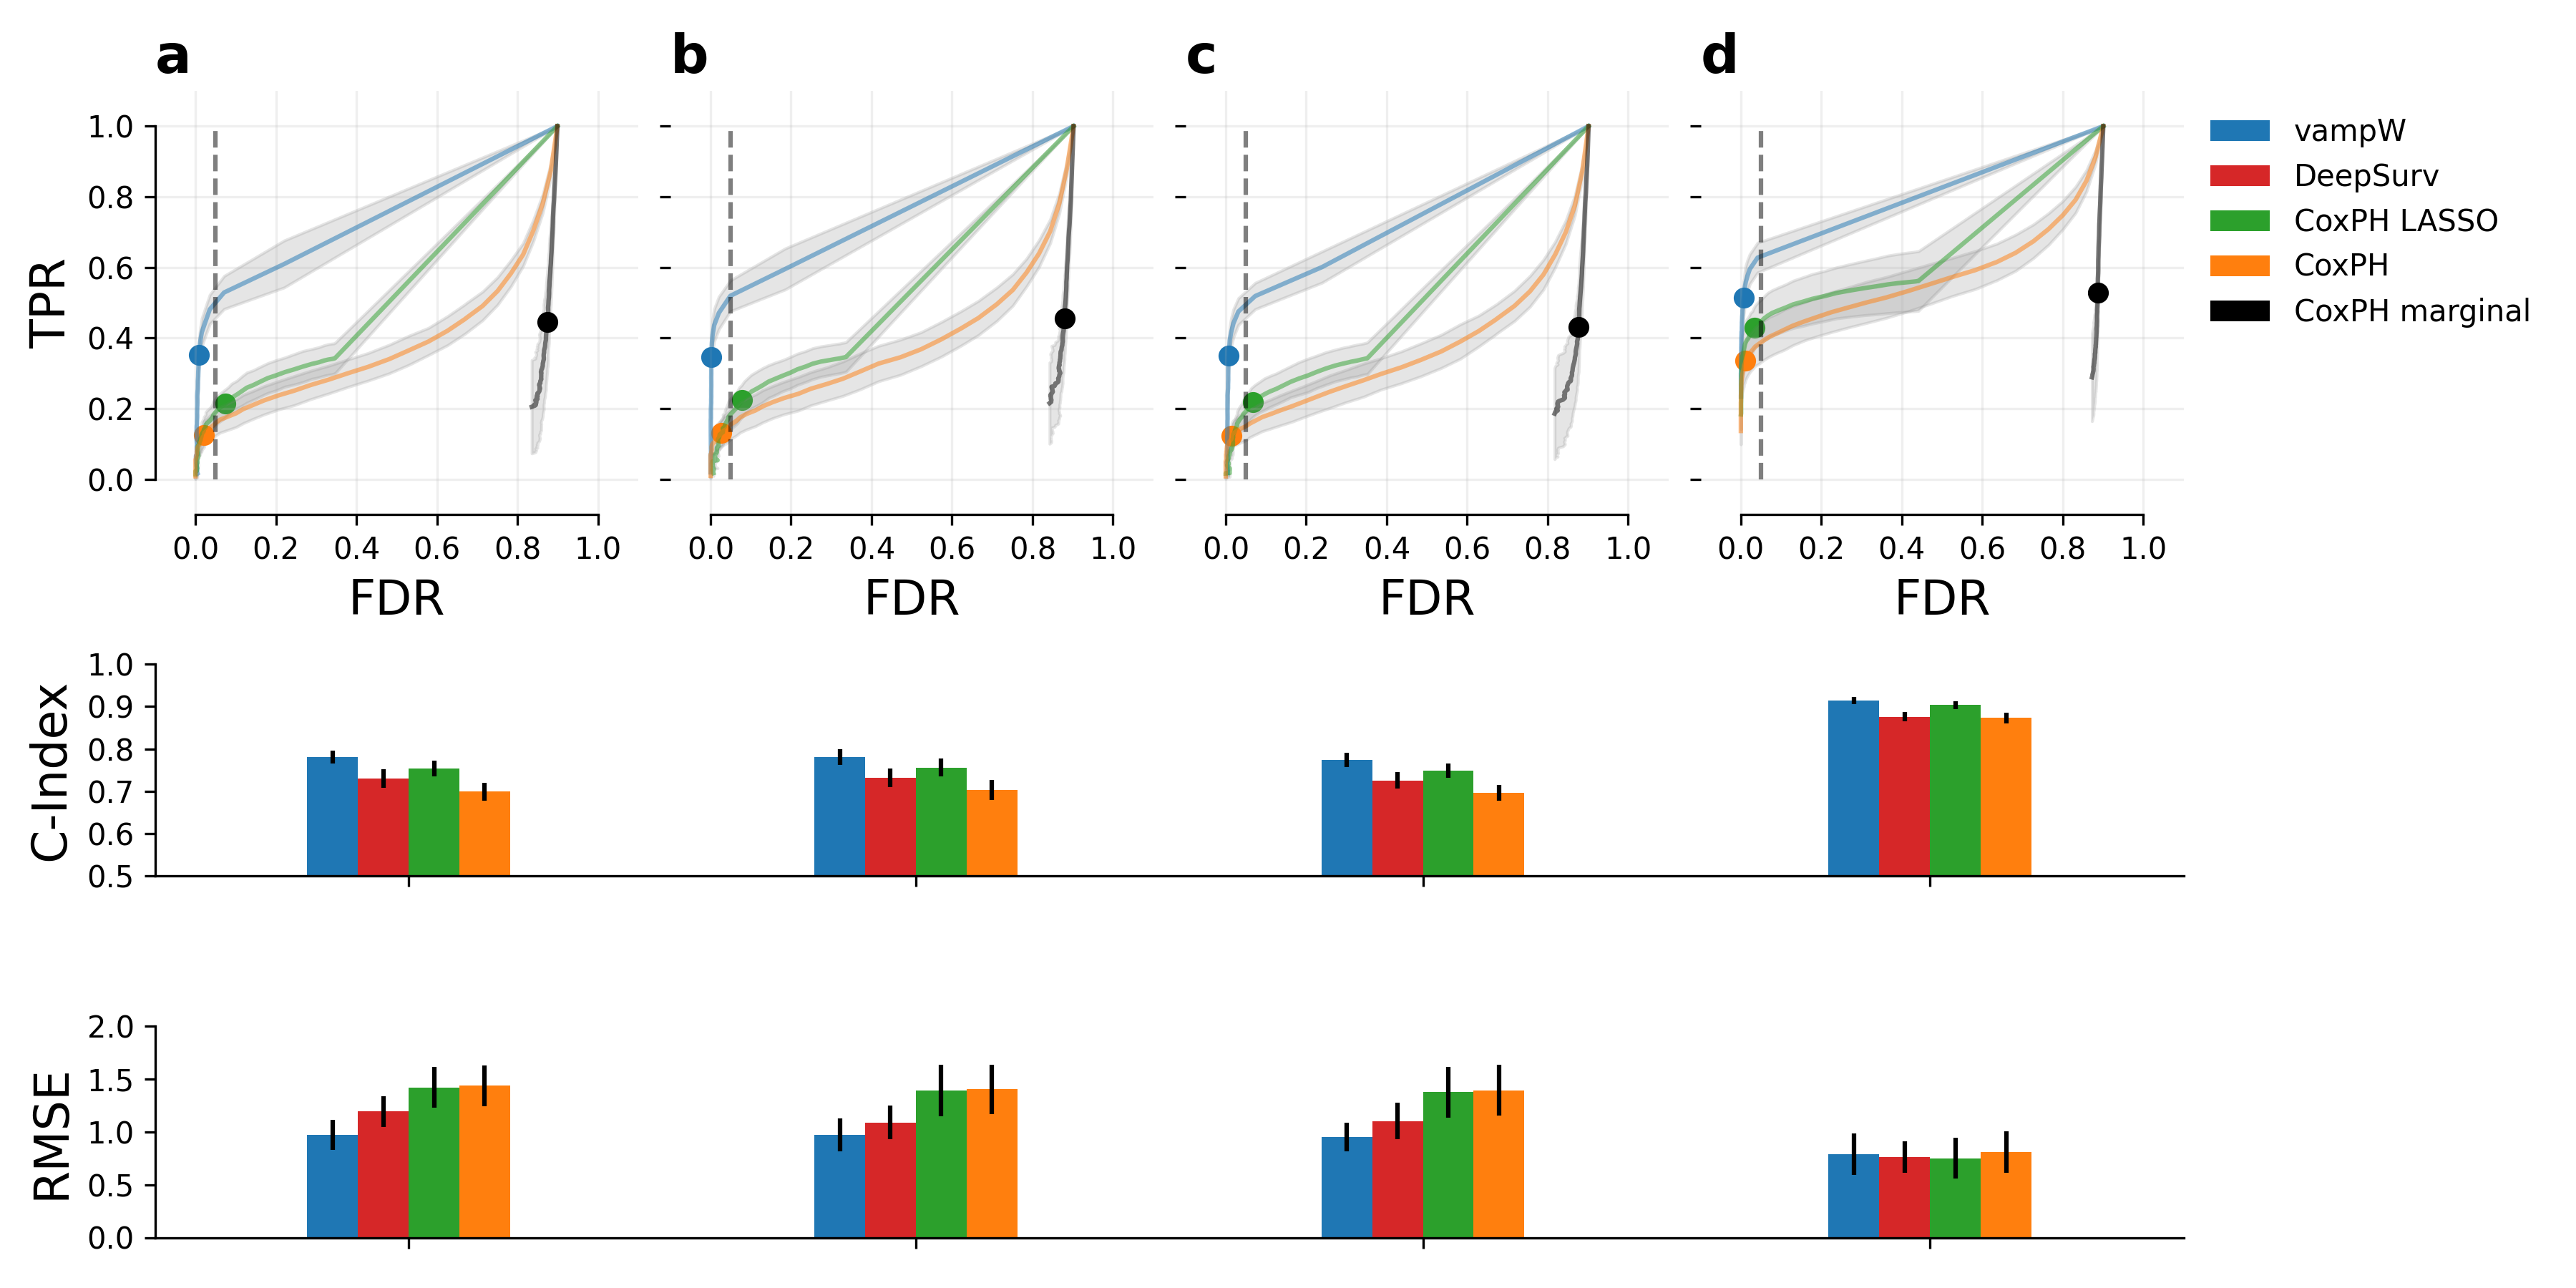
\includegraphics[width=\linewidth]{figures/panel_plot_1.png}
    \end{center}
    \caption[Simulation study of variable selection and out-of-sample prediction performance using 2,924 proteins across 53,018 individuals from the UK Biobank]{
    \textbf{Simulation study of variable selection and out-of-sample prediction performance using 2,924 proteins across 53,018 individuals from the UK Biobank.} We present four representative simulation scenarios (out of the 24 in total presented in Supplementary Figures~\ref{fig:fdr_tpr}-\ref{fig:sim_paired_differences}), covering low signal-to-noise ratios, model mis-specification, and high censoring rates. Specifically, subplots (a, b, c, d) correspond to simulation scenarios (m, o, q, t), as described in Supplementary Table \ref{tab:sim}. Across all subplots, we use the following color convention: vampW in blue, marginal CoxPH in black, joint CoxPH in orange, LASSO-penalized CoxPH in green, and DeepSurv in red. In the first row, we show variable selection performance as the relationship between \acrlong{fdr} ($\text{FDR} = \text{FP} / (\text{FP} + \text{TP}))$  and true positive rate ($\text{TPR} = \text{TP} / (\text{TP} + \text{FN}))$. For vampW, we use posterior inclusion probabilities (PIPs), while for the other methods, p-value testing across multiple thresholds is employed, see Methods for details. Colored dots indicate the 0.95 threshold for vampW PIP and the Bonferroni-corrected 0.05 threshold for the other methods. The second row presents prediction performance measured by the concordance index (C-index) on a held-out test set. The last row presents prediction performance measured by the Root Mean Squared Error (RMSE) between the true and predicted survival times in the logarithmic domain, on uncensored individuals. The error bars (black lines in the bar plots and gray shaded areas in FDR-TPR plots) represent the standard deviation across 50 simulation replicates. \label{fig:main1}} 
\end{figure}

We begin by benchmarking vampW against several state-of-the-art variable selection approaches within a semi-synthetic simulation study. Using the 2,924 observed protein levels from the UKB PPP dataset measured in 53,018 individuals, we simulate artificial phenotypic outcomes in 24 scenarios (see Methods for details). The varied parameters are: \emph{(i)} the proportion of variance explained by biological markers, \emph{(ii)} the proportion of censored individuals, \emph{(iii)} the phenotype distribution (Weibull, ExpGamma), \emph{(iv)} the prior distribution of the slab part of the regression coefficients (Normal, Laplace), and \emph{(v)} the ExpGamma distribution parameter. Each scenario is repeated 50 times to obtain independent realizations of the simulated data, and train/test splits are resampled at a 90\%/10\% ratio across these realizations. We evaluate vampW against several approaches: one-protein-at-a-time testing (CoxPH marginal); non-penalized CoxPH fitted to all markers jointly (CoxPH); joint LASSO-penalized CoxPH with cross-validation and stability selection (CoxPH LASSO); and the deep learning approach DeepSurv (see Methods for details). We assess the ability of each method to recover the simulated causal variables and the out-of-sample time-to-event observation prediction accuracy. For variable selection, we report the false discovery rate (FDR) and true positive rate (TPR) in 4 representative scenarios in Figure \ref{fig:main1}, where $\text{FDR} = \text{FP} / (\text{FP} + \text{TP})$ and $\text{TPR} = \text{TP} / (\text{TP} + \text{FN})$, with $\text{FP}$ denoting number of false discoveries, $\text{TP}$ the number of true positive discoveries, and $\text{FN}$ the number of false negative discoveries. FDR–TPR plots for all 24 simulation scenarios are reported in Supplementary Figure~\ref{fig:fdr_tpr}.

The results of Figure \ref{fig:main1} show that joint variable selection under the Weibull model of our vampW approach achieves a calibrated false discovery rate, while outperforming both marginal and joint CoxPH models in terms of true positive rate. More precisely, marginal one-at-a-time association testing using the Cox model produces over 80\% false positives across all simulated scenarios, even with a Bonferroni correction. This is due to the fact that, when testing each protein individually, correlations can inflate false discoveries as the estimated effect is confounded by other correlated proteins. Modeling the data using a single joint CoxPH model substantially reduces false positives, leading to well-calibrated association testing with a false discovery rate below 0.05\%. Joint approach reduces the pool of candidate markers for clinical testing while capturing combined or conditional effects, which may be more informative for understanding biological pathways. Furthermore, employing a LASSO-penalized CoxPH model with 5-fold cross-validation and stability selection increases power over the joint CoxPH model, while maintaining a well-calibrated false discovery rate in most scenarios. However, the TPR achieved by the LASSO-penalized CoxPH model with stability selection is still lower than that of vampW across all settings. The complete results for all the 24 simulation scenarios in Supplementary  Figure~\ref{fig:fdr_tpr} are similar to those presented in Figure \ref{fig:main1}, where overall, the TPR of vampW is higher, with comparable or improved FDR to CoxPH approaches. This holds even under model mis-specification (generalized Gamma distribution with shape parameter $\kappa \in \{0.8, 1.2\}$) or when the prior distribution of simulated regression coefficients follows a spike-and-slab prior with slab component being a Laplace distribution which has heavier tails than the Gaussian slab prior used by vampW (Supplementary Figure~\ref{fig:fdr_tpr}). 
 
We investigate the ability of vampW to recover signals from highly correlated proteins, by annotating proteins based on their correlation structure (the top 100 correlated proteins are shown in Supplementary Figure~\ref{fig:correlation}). If the correlation of a particular protein with any other protein is greater than 0.5 in terms of the absolute value of the Pearson correlation coefficient, it is categorized as a highly correlated protein, with remaining proteins categorized as low-correlated. Supplementary Figure~\ref{fig:annot} shows that, among true-positive predictions with PIP $\geq$ 0.95, the fraction of highly versus low-correlated proteins closely matches the corresponding fraction among ground-truth in the simulation. Thus, vampW has equivalent detection power across proteins of different correlation structure.

We then compare the out-of-sample prediction accuracy across approaches, using two metrics: \emph{(i)} Harrell's concordance index (C-index) \cite{harrell_evaluating_1982}, which measures the proportion of concordant pairs, defined as $\text{C-index}=(n_{c} + 0.5 \cdot n_t) / n_{a}$, where $n_{c}$ is the number of pairs which are in the same order in predictions in comparison to the observation, $n_{t}$ is the number of tied pairs, and $n_{a}$ is all possible admissible pairs; and \emph{(ii)} root mean squared error (RMSE), which represents the average error between the predicted times and the actual diagnosis times for uncensored individuals, defined as $\text{RMSE}(\bm{y}, \hat{\bm{y}})= (N^{-1} \sum_{i=1}^{N} (y_i - \hat{y}_i)^2)^{1/2}$, where $\hat{\bm{y}}$ is the predicted outcome time and $\bm{y}$ is the ground-truth for the uncensored individuals. For the simulation results (Figure~\ref{fig:main1} and Supplementary Figures~\ref{fig:sim_prediction} and ~\ref{fig:sim_paired_differences}), the RMSE is computed on $\log(\bm{y})$, which is the quantity standardized to zero mean and unit variance by all methods. For the results on real data (Figure~\ref{fig:main3}), the RMSE is computed on $\bm{y}$, which represents the actual time of onset and hence provides a more interpretable quantity.

Prediction accuracies for different methods are presented in Figure~\ref{fig:main1} for 4 representative scenarios, in Supplementary Figure~\ref{fig:sim_prediction} for all 24 simulation scenarios and in Supplementary Figure~\ref{fig:sim_paired_differences} considering pairwise differences of these performance metrics across different simulation replicas. These plots show that, in comparison to CoxPH LASSO, vampW achieves higher C-index values across all simulation scenarios, as well as lower or on par RMSE in all scenarios. We additionally compare vampW to DeepSurv, a deep learning extension of the CoxPH model developed for risk prediction. DeepSurv performs better than the standard CoxPH, but is outperformed by vampW in all simulation scenarios in terms of C-index. In terms of RMSE, in most simulation scenarios vampW and DeepSurv exhibit similar performance, with vampW being significantly better in three scenarios. We refrain from comparing association testing performance that of DeepSurv, as the latter was primarily developed for prediction tasks (in which it does not improve upon vampW) and it does not provide variable selection within the current framework. 

\subsection{Analyzing 24 disease-related outcomes in UK Biobank}

\begin{figure}[t]
    \begin{center}
    \includegraphics[width=\linewidth]{figures/panel_plot_2.png}
    \end{center}
    \caption[Protein-coding genes discovered by vampW and their genomic positions]{\textbf{Protein-coding genes discovered by vampW and their genomic positions.} The proteins discovered by vampW and their corresponding protein names that pass a posterior inclusion probability (PIP) threshold of 0.95 are shown. Disease outcomes are categorized into four groups: neurological diseases, cardiovascular diseases, cancer types, and other disease-related outcomes.\label{fig:main2}}
\end{figure}

We apply vampW to the age-at-diagnosis of 24 disease outcomes derived from medical records in the UK Biobank, linked to protein measurements from blood samples. \changed{In Figure \ref{fig:main2}, we report two sets of vampW discoveries, passing a PIP threshold of 0.95, for models with and without exponential age correction. First, for the model without exponential age correction, we also run marginal CoxPH, joint CoxPH, and LASSO-penalized CoxPH analyses, all using Bonferroni-corrected p-value testing.} Marginal testing identifies tens of times more associations compared with joint vampW testing, consistently across most traits (exceptions being Alzheimer’s disease, vascular dementia, brain/CNS disorders, and prostate disease). However, our simulation study indicates substantial inflated false discoveries when using marginal testing, which often selects features that appear significant individually but are correlated with each other, whereas joint testing produces a potentially more biologically meaningful set of discoveries, reducing the need for unnecessary follow-up experiments. The set of vampW discoveries is largely independent of the top-$x$ marginal discoveries, where $x$ corresponds to the number of vampW discoveries. Specifically, the overlap between vampW and the top-$x$ marginal CoxPH results is 37 out of 219 vampW associations. This indicates that vampW identifies largely novel associations, and that its joint testing capability cannot be replicated simply by tightening the marginal testing p-value threshold. In comparison with joint CoxPH and LASSO-penalized CoxPH, 61 and 110 associations, respectively, overlap with vampW. The overlap indicates that vampW is not overly conservative in variable selection, as it identifies proteins that are also detected by LASSO. For 9 of the 24 traits, no association passes the PIP threshold.

In the set of discoveries without exponential age correction, we highlight the discovery of collagen alpha-1(IX) \emph{COL9A1} in type 2 diabetes, which was also identified by the standard joint CoxPH model but not by CoxPH LASSO. Although it has previously been reported among top plasma proteins \cite{deng_atlas_2025}, it is not well established as a biomarker and may provide novel insights into the biological pathways underlying the disease. Another potentially novel association with type 2 diabetes is the \emph{MATN3} gene, which also exhibits an underlying interaction with \emph{COL9A1} based on text mining, as shown in Supplementary Figure~\ref{fig:interaction_networks}. Furthermore, we identify \emph{SOST} as a novel candidate associated with endometriosis, a potential biomarker that has not been widely studied in this context.

One of the leading associations we identify is the protein-coding gene \emph{CGA}, which is associated with multiple diseases, including endometriosis, T2D, depression, ischemic heart disease, liver disease, Parkinson’s disease, gynecological cancer, prostate cancer, and colorectal cancer. Notably, plasma levels of \emph{CGA} are highly influenced by age and sex in non-linear ways and rank among the top six protein-coding genes (alongside \emph{FSHB}, \emph{SOST}, \emph{GDF15}, \emph{MLN}, and \emph{PTN}) exhibiting the most significant age-dependent changes \cite{deng_atlas_2025,Sigurdsson2025}. This suggests that plasma levels of these proteins may be associated with these outcomes simply because both the proteins and the time-to-diagnosis both vary exponentially with age. 

To explore this further, we conduct an additional adjustment of the plasma protein observations including exponential age effects along with the linear ones (see Methods), and re-analyze the traits. This yields associations of plasma protein levels with disease onset beyond age-related variation. The protein-coding gene \emph{CGA}, previously reported as age-associated, disappears from ischemic heart disease, colorectal disease, and mortality associations when non-linear effects of age on protein levels are taken into account (see Figure~\ref{fig:main2} and Figure~\ref{fig:cov_age}). Moreover, for certain outcomes, the signal becomes attributed to a different set of proteins, revealing new underlying biological structure. For example, we find the chemokine \emph{CXCL17} as associated with colorectal cancer, which is previously reported as a potential biomarker for the diagnosis of colon cancer \cite{ohlsson_ectopic_2016}. Furthermore, we identify Tenascin-XB (TNXB) protein, encoded by the TNXB gene, which is recognized as a potential blood-based plasma biomarker associated with depression \cite{biomedicines8110455}. PARK7 (also known as DJ-1) is a multifunctional protein that acts as an antioxidant sensor. Its oxidized form (oxDJ-1) in blood has been proposed as a promising biomarker for early-stage Parkinson’s disease \cite{Matsuda2024ModificationsOD}. It was also identified by vampW, after exponential age correction, in association with Parkinson’s disease and rheumatoid arthritis.

Regardless of the age correction approach, we find several associations supported by recent literature. In particular, we find \emph{ACE} to be associated with both hypertension and ischemic heart disease, supporting a role in blood pressure regulation \cite{zambrano_genetic_2023}. Prostate-specific antigen (PSA) is the most widely used clinical biomarker for identifying men at risk of prostate cancer prior to symptom onset, and its mechanisms have been extensively studied \cite{pellegrino_mechanistic_2021}. PSA is encoded by the \emph{KLK3} gene, which exhibits an association with prostate cancer, regardless of age correction approach in our study. Growth differentiation factor 15 (\emph{GDF15}) reduces food intake and represents a promising therapeutic target for the treatment of type 2 diabetes \cite{aguilar-recarte_knocking_2022}. It is also a useful biomarker for identifying individuals at increased risk of diabetes \cite{aguilar-recarte_knocking_2022}, and vampW exhibits a strong association between GDF15 protein levels and type 2 diabetes. Variation in the \emph{APOE} protein, especially the alleles $\varepsilon_3$ and $\varepsilon_4$, has been widely established as a risk factor for late-onset disease across multiple large cohorts \cite{williams_proportion_2026}. Regardless of adjustment for non-linear age effects, we find \emph{APOE} to be significantly associated with Alzheimer’s disease progression. \changed{We also identify renin (REN) associated with hypertension, which is a key enzyme in the renin-angiotensin-aldosterone system (RAAS), making its measurement—often via plasma renin activity (PRA)—a crucial biomarker for classifying, diagnosing, and assessing cardiovascular risk in hypertension patients \cite{VOLPE2012312}.}

% Overall, vampW discoveries exhibit average replication rates across traits of 52\% and 73\% for models with and without exponential age correction, respectively, when compared with the DISEASES 2.0 gene–disease database at a Z-score threshold of 2, adjusted for overlap in genes and diseases between the datasets. 
We further identify 262 and 9 protein associations, respectively, for the models with and without exponential age correction that show no prior link to a given disease in the DISEASES 2.0 database, which integrates disease-gene associations from automatic text mining and is updated on a weekly basis (we use March 2026 version). We examine the total \acrfull{snp} heritability of proteins, as shown in Supplementary Figure \ref{fig:protein_h2}, using values reported in \cite{sun_plasma_2023}. We find no significant deviation of vampW-discovered proteins compared to all proteins in the study, with average SNP heritability of 19.9\% and 18.7\% for models with and without exponential age correction, respectively.

To further validate the vampW discoveries and assess whether they can be replicated in a cohort using a different sampling technology, we matched proteins and outcomes between the UK Biobank and a SomaScan v4 study of plasma samples from 36,000 Icelandic individuals \cite{eldjarn_large-scale_2023}.
% To further validate the vampW discoveries, we match proteins and outcomes between the UK Biobank and a SomaScan v4 study of plasma samples from 36,000 Icelandic individuals \cite{eldjarn_large-scale_2023}. 
Among the vampW discoveries, we identified matching proteins for Alzheimer's disease, depression, hypertension, rheumatoid arthritis, and prostate cancer. Of the 71 matched discoveries, 48 also show an association using logistic regression with binary disease occurrence in the Icelandic cohort at a Bonferroni-adjusted p-value threshold. 
% Moreover, we attempted to replicate our findings in the independent Generation Scotland (GS) study, which employed SOMAscan V.4 technology, in contrast to the Olink Explore 3072 PEA platform used in UK Biobank. We observed limited overlap in the proteins measured across the two studies, as well as a low prevalence of certain diseases of interest, making replication challenging. Nevertheless, we successfully replicated the association of CDH5 with hypertension, a protein recently recognized as a key contributor to hypertension pathogenesis \cite{aldisi_identification_2025}.

\begin{figure}[t]
    \begin{center}
    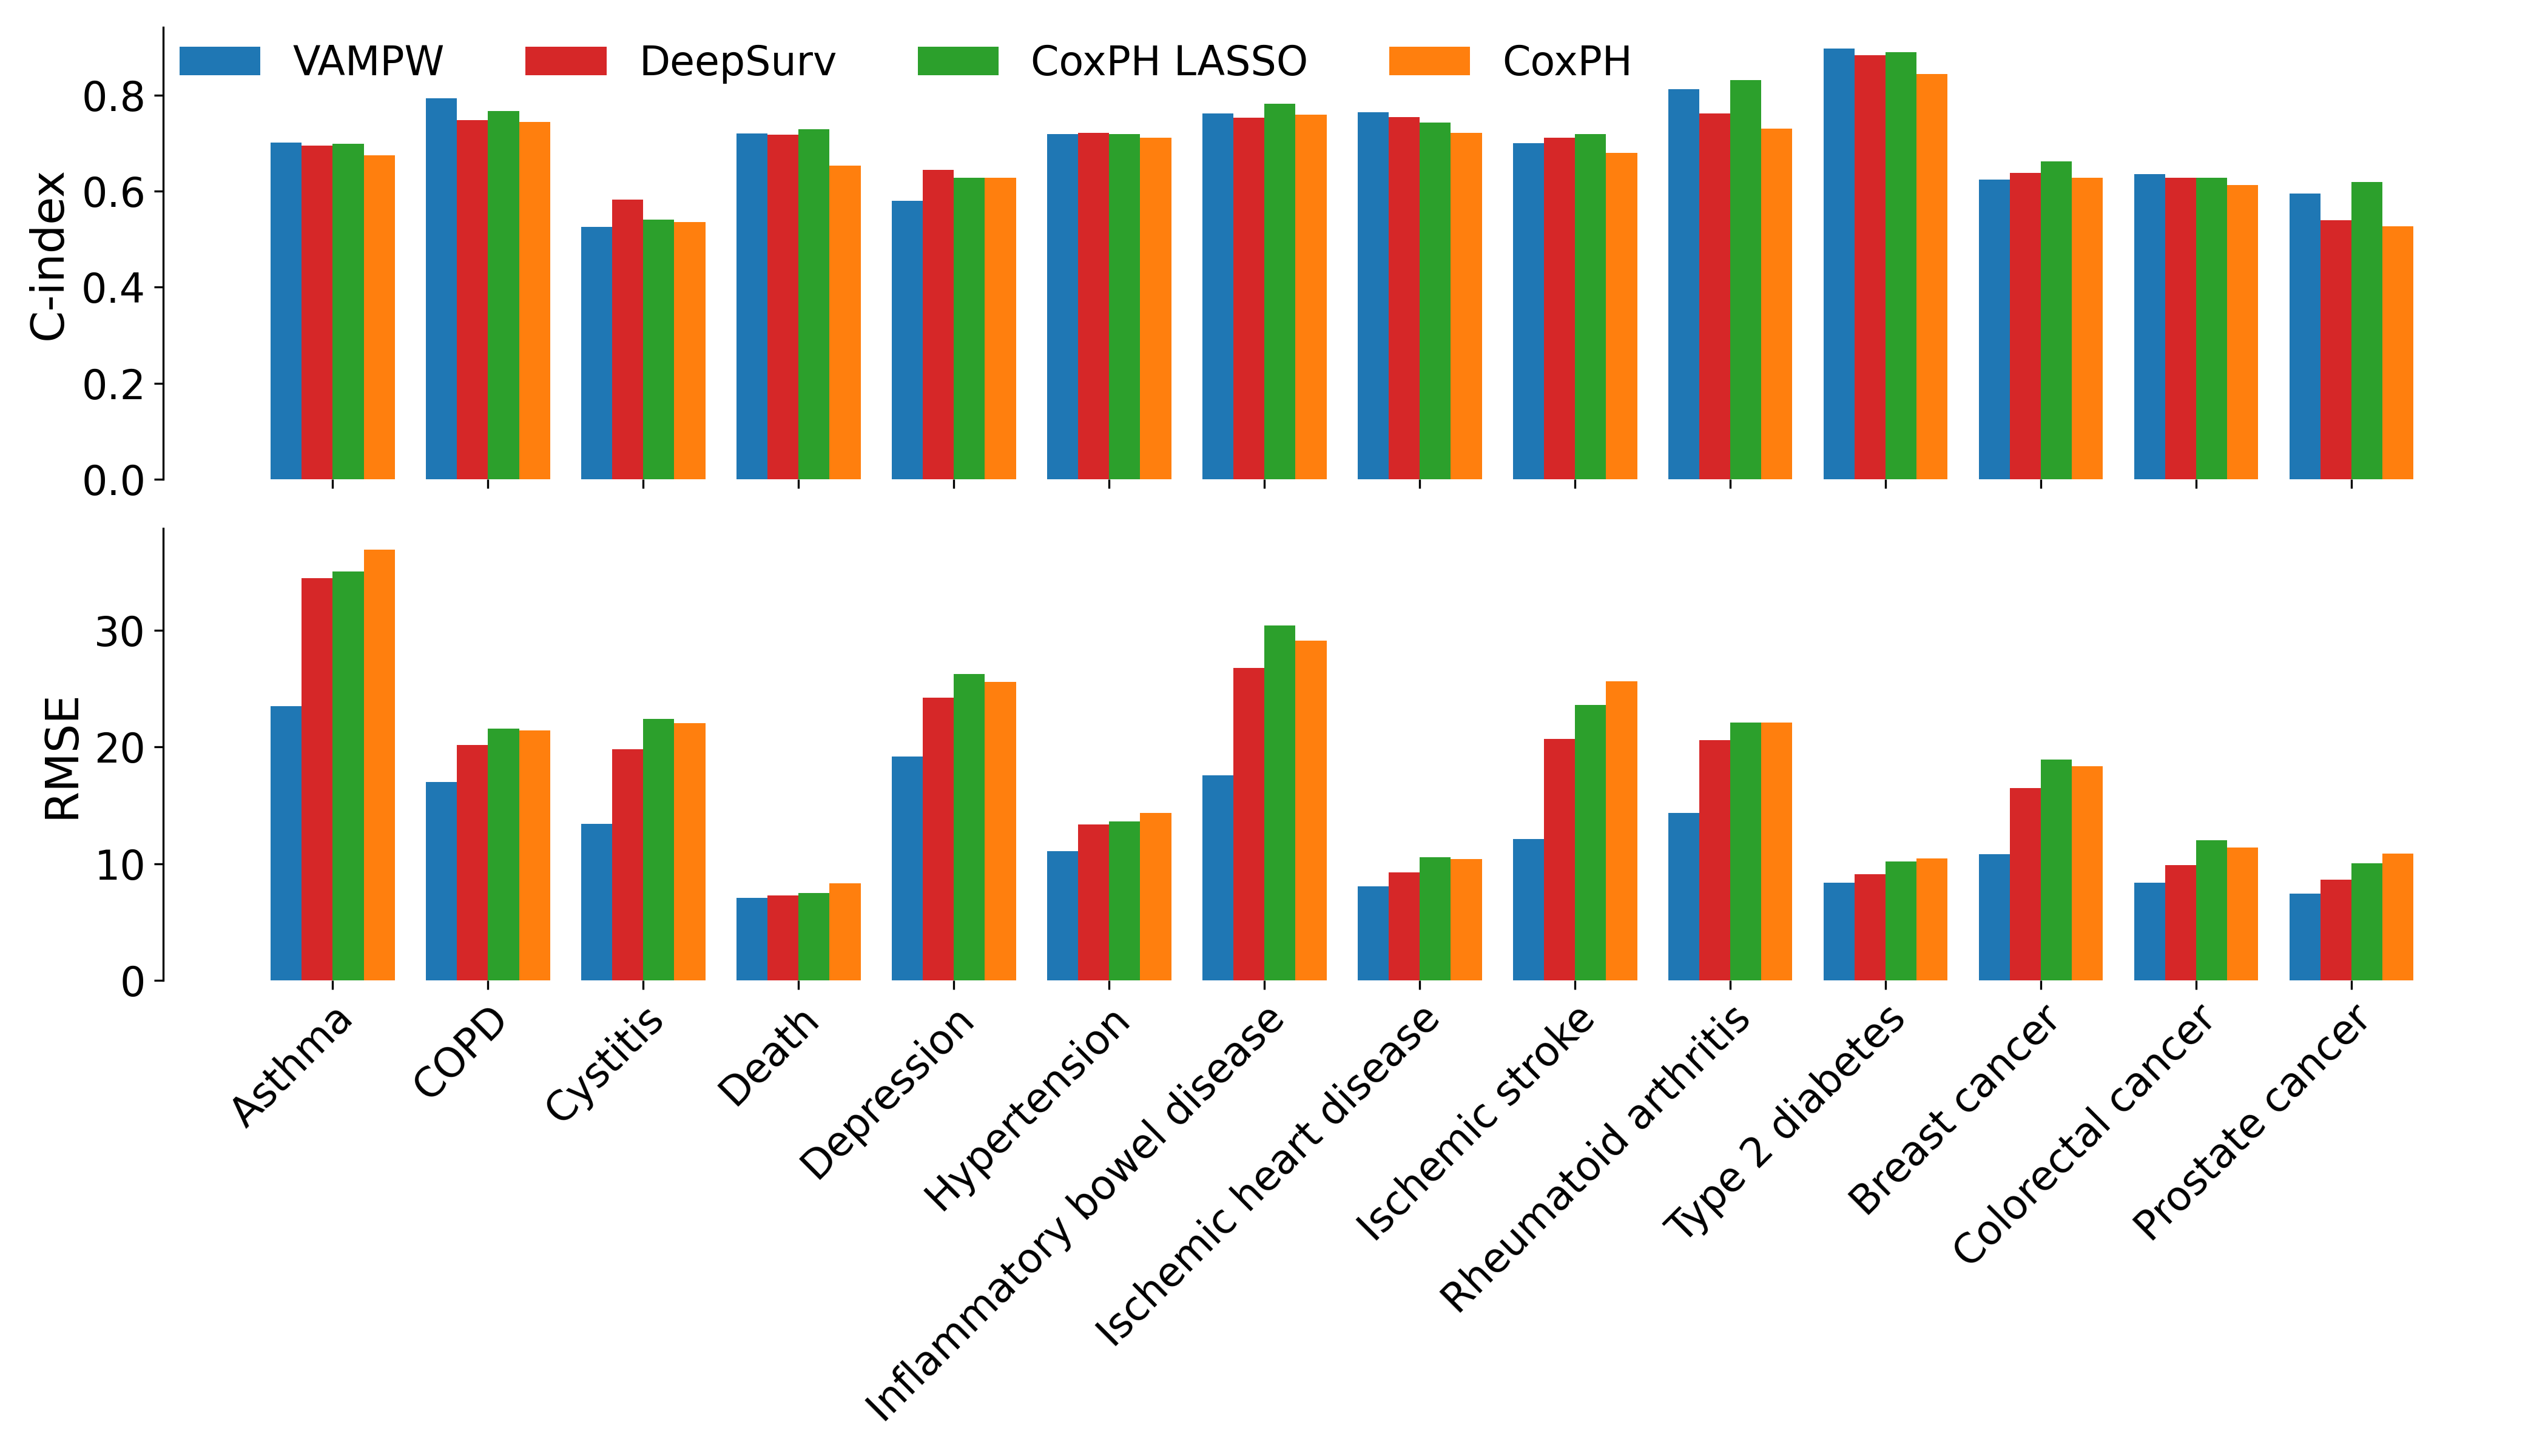
\includegraphics[width=\linewidth]{figures/panel_plot_3.png}
    \end{center}
    \caption[Out-of-sample performance comparison for CoxPH, LASSO-penalized CoxPH, DeepSurv, and vampW]{
    \textbf{Out-of-sample performance comparison for CoxPH, LASSO-penalized CoxPH, DeepSurv, and vampW.} 
    We evaluate time-to-diagnosis predictions for 14 health-related outcomes in the UK Biobank (traits with $\ge 100$ cases in the test set) using protein measurements adjusted for age and sex. 
    Model accuracy is assessed using the Concordance Index (C-index), which measures the probability of correctly ranking patient risks, and the root mean squared error (RMSE), representing the average error in years between predicted and actual diagnosis times for uncensored individuals. Training is performed on data that is first log-transformed and standardized to zero mean and unit variance, and then scaled back using an exponential transformation. To represent actual survival times, we rescale the predictions back to years using statistics from the training set. A sensitivity analysis shows that using test-set statistics for this rescaling impacts results negligibly and preserves the ordering of methods in terms of their performance. In terms of RMSE, vampW significantly improves over all other methods. In terms of C-index, vampW outperforms CoxPH, and it performs on par with CoxPH LASSO and DeepSurv.
  }
    \label{fig:main3}
\end{figure}

In Figure \ref{fig:main3}, we show the absolute values of C-index and RMSE metrics across traits with more than $100$ uncensored individuals (representing cases) present in the test set. In terms of RMSE, vampW outperforms all other methods across all traits: on average, it reduces the RMSE by 33\% with respect to CoxPH, by 32\% with respect to CoxPH LASSO and by 26\% with respect to DeepSurv. Figure~\ref{fig:main3} gives the RMSE in the actual scale of years, and we also present the RMSE in the logarithmic time domain, assuming standardized $\log(\bm{y})$, in Supplementary Figure~\ref{fig:real_rmse_time}, which shows that the relative performance ranking of the methods remains unchanged.

In terms of out-of-sample C-index performance, vampW shows an improvement over CoxPH in $11/14$ traits, over LASSO-penalized CoxPH in $6/14$ traits and over DeepSurv in $9/14$ traits. Furthermore, on average, the C-index of vampW is 0.5\% better than that of DeepSurv, 4\% better than that of CoxPH, and 1.3\% worse than that of LASSO-penalized CoxPH. Finally, we note that the largest deviations from the Weibull distribution, as shown in Supplementary Figure \ref{fig:distance}, occur for asthma and inflammatory bowel disease, for which vampW has limited power for association testing but still demonstrates improved time-prediction performance over the various baselines. In comparison to other methods, vampW yields better prediction performance at later ages for most outcomes, based on the Brier score, as shown in Supplementary Figure~\ref{fig:bs_t75}.

We find that vampW generates highly transferable protein risk scores across diverse genetic ancestries, maintaining predictive utility in minority populations. Specifically, while vampW achieves comparable accuracy in terms of C-index to CoxPH LASSO, it consistently outperforms both standard CoxPH and CoxPH LASSO models in minimizing overall prediction error (RMSE), as seen in Supplementary Figure~\ref{fig:genetic_ancestry_exp_50_10}.

To demonstrate the wider applicability of our algorithm outside the proteomics domain, we additionally benchmark vampW in data-scarce regimes using common survival benchmarking datasets, following the study \cite{monod_neuralsurv_2025}. As shown in Supplementary Figure~\ref{fig:deep_benchmark}, vampW outperforms all deep learning methods on the METABRIC, SUPPORT, and SAC3 datasets, and outperforms 6 out of 13 benchmarking methods on the GBSG dataset. 

\section{Discussion}
In this work, we develop the novel vampW algorithm for Bayesian variable selection under the Weibull model. Applying our approach to the largest proteomics data available to date, we demonstrate its capability to jointly fit thousands of plasma proteomics markers across tens of thousands of individuals from the UK Biobank, revealing new disease biomarkers. Our simulation study shows that vampW outperforms state-of-the-art methods for variable selection, reducing false discoveries compared to marginal testing and improving the true positive rate relative to multiple forms of CoxPH models. When analyzing real health-related outcomes from the UK Biobank, vampW identifies 219 associations between protein levels and human complex diseases. Our discoveries exhibit a 68\% replication rate in an independent Icelandic cohort, accounting for overlap in proteins and outcomes between the studies. 

vampW provides point estimates of the posterior mean, and its prediction performance is expected to be Bayes-optimal. For out-of-sample prediction of the outcome ranking (C-index), vampW outperforms the standard CoxPH model and achieves performance comparable to penalized versions of CoxPH and to the deep learning-based method DeepSurv. For the prediction of disease onset times in uncensored individuals, vampW yields more accurate predictions, measured by RMSE, as compared to all other benchmarked methods. We also show that vampW generates highly transferable protein risk scores across diverse genetic ancestries and achieves strong out-of-sample prediction performance in other non-proteomics data-scarce regimes, outperforming deep learning methods on most of the examined survival benchmarking datasets, even when trained on very small sample size. 

There are several limitations and potential avenues for future work. First, plasma protein levels, as well as other multi-omics markers, may be influenced by multiple confounding factors, such as medication use, sex, and age, including non-linear effects of age on protein levels, as suggested by our ablation study. In this context, a key direction for future work is to leverage the medical records of individuals in the UK Biobank, which would allow adjustments for a broader set of potential confounders. Moreover, to examine whether variation in protein levels reflects disease predisposition or the disease state itself, one possible approach is to restrict the analysis to individuals who experience events after the date of blood sampling and assessment, rather than incorporating both prospective and historical events. With more samples available, covering a larger portion of the population prevalent with a certain disease, studying associations between survival time and protein levels during the follow-up period represents a viable approach. Additional extensions are models that can identify relevant age-related changes in protein levels that are associated with disease onset at different time points, which requires repeated proteomics observations.

In terms of model stability, although the UKB PPP protein design matrix violates the assumptions required for Bayes optimality of our algorithm, introducing damping and damping autotuning (see Methods) empirically results in strong predictive performance. The damping choices affect the convergence properties when searching over the parameter space, as too strong damping may cause the algorithm to get stuck in local minima; and thus we propose a grid search of starting parameters which is facilitated by the efficient implementation of our algorithm (see Methods). 

% \marco{this paragraph does not seem to belong here, but would be better suited for Methods?}


Finally, our future work will also focus on improving the computational efficiency of the vampW algorithm through parallelization and reduced memory requirements, which has the potential to enable large-scale analyses involving hundreds of thousands of omics markers.  

In summary, vampW is a novel approach for selecting multiomic biomarkers associated with human diseases and for predicting disease onset times. With increasing sample sizes and expanding data coverage in the world’s largest biobanks, joint vampW analyses have the potential to advance our understanding of the genomic architecture of complex human diseases by enabling interpretable identification of disease associations and providing accurate predictions of disease onset.

\section{Methods}
\subsection{Weibull model for time-to-event outcomes}\label{subsec:W}

We consider a Weibull$(\alpha, \eta)$ model, one of the most common models in survival analysis, where $\alpha$ and $\eta$ are the shape and scale parameters. We follow a recently proposed formulation of the model~\cite{Ojavee2021-zu}, where we aim to estimate mean and variance of the time-to-event outcome. Let $y_i$ be the time at which the individual $i$ experiences the event, and consider the survival function $S(y_i) = \exp(-(\frac{y_i}{\eta_i})^{\alpha})$. In the logarithmic space, the mean and variance of the model can be separated as follows:
\begin{align}
    & \mathbb{E}[\log(y_i)] = \log(\eta_i) - \frac{K}{\alpha}, \\
    & \text{Var}[\log(y_i)] = \frac{\pi^2}{6 \alpha^2},
\end{align}
where $K$ is the Euler-Mascheroni constant ($\approx 0.57722$). Once the variance is independent of the scale parameter $\eta_i$, one can introduce the vector of underlying latent genetic effects $\bm{\beta}$ as $\bm{\eta} = \exp(\mu + \bm{X} \bm{\beta} + \frac{K}{\alpha})$, resulting in $\mathbb{E}[\log(\bm{y})] = \mu + \bm{X} \bm{\beta}$, where $\bm{X} \in \mathbb{R}^{N \times P}$ is a design matrix containing observations on $N$ individuals and $P$ biological markers, $\bm{y}=[y_1, \ldots, y_N]$, $\bm{\eta}=[\eta_1, \ldots, \eta_N]$, $\bm{\beta}$ is the vector of marker effects, and $\mu$ represents the model intercept. The columns of the matrix $\bm{X}$ are normalized, i.e., they each have zero mean and unit variance. Using the fact that the logarithm of a Weibull random variable follows a Gumbel distribution and the Location-Scale property of the Gumbel distribution, we formulate the final model as
\begin{equation}
    \label{eq:vampW_model}
    \log (\bm{y} )=\mu + \bm{X} \bm{\beta} + \frac{\bm{w}}{\alpha} + \frac{K}{\alpha}, 
\end{equation}
where $\bm{w} = [w_1, \dots, w_N]$ with each $w_i$ following the Gumbel$(0,1)$ distribution. We note that in the algorithm and software described below, any arbitrary measurement represented in floating point can be accommodated as the entries of $\bm{X}$. These can be gene expression, methylation, copy number variants, DNA sequence variation, protein measures, which can all be included alongside one another. 

To allow for a range of effect sizes from different data types, we select the prior on the marker effects $\bm{\beta}$ to be distributed as a form of spike and slab distribution, with non-zero signals coming from a mixture of normal distributions,
\begin{equation}
\label{eq:prior}
    \beta_j \sim ( 1 - \lambda ) \delta_0 + \lambda \sum^L_{i=1} \pi_i \cdot \mathcal{N}(0, \sigma^2_i),
\end{equation}
where $(\pi_1, \dots, \pi_L)$ denotes the vector of inclusion probabilities for each of the $L$ mixture components, $\delta_0$ is a Dirac spike function at 0, $\lambda$ is the sparsity ratio, and $(\sigma^2_1, \dots, \sigma^2_L)$ are mixture-specific variances.

Finally, we account for the right-censoring issue inherent in time-to-event data. In practical applications, the true event time $y_i$ is often right-censored, meaning that the event of interest has not occurred for some individuals by the end of the study. Consequently, we do not observe $y_i$ directly for all $i$; instead, we observe the time $\min(y_i, C_i)$ and an indicator $\delta_i = \mathbb{I}(y_i \leq C_i)$, where $C_i$ is the censoring time and $\delta_i=1$ implies the event was observed while $\delta_i=0$ implies it was censored.

\subsection{vampW algorithm and its implementation}\label{sec:vampW}

To infer the parameters of Equations \eqref{eq:vampW_model} and \eqref{eq:prior}, we propose an algorithm that we call vampW, which is based on Vector Approximate Message Passing (VAMP) for generalized linear models \cite{rangan_vector_2019, schniter_vector_2016}, where the outcome variable is observed through a noisy and non-linear Weibull channel. It adaptively estimates the prior-specific parameters $\Theta = \{\lambda, (\pi_i)_{i=1}^L, (\sigma_i^2)_{i=1}^L \}$ via a Bayesian Expectation-Maximization procedure, as introduced in EM-VAMP \cite{LearningFreeEnergies2018}. vampW introduces a novel approach for handling censored data, as well as denoisers derived specifically for Weibull link functions and the corresponding expectation-maximization updates. We highlight that no existing AMP method is able to address the challenge of censored data. 
% \marco{unnatural rendering: lots of blank space in this page and in the next page the page number displays in the middle of the algorithm. Please fix.}

As seen in Algorithm \ref{alg:vampW}, vampW consists of two denoising steps and two (non-linear) minimum mean-squared error (MMSE) estimation steps, applied separately to the vector of effect sizes $\bm{\beta}$ and to the latent predictor. The denoising step accounts for the prior properties of the model when considering a noisy estimate of either  $\bm{\beta}$ or the latent predictor, while the MMSE step further refines the estimates by taking the correlation structure among the columns in the design matrix $\bm{X}$ into account. The key feature is the so-called \textit{Onsager correction}, which is added to ensure the asymptotic normality of the noise corrupting the algorithm's estimates of $\bm{\beta}$ at every iteration, important for the subsequent feature selection. A direct application of generalized EM-VAMP to real genomics, epigenetics and proteomics measures may lead to signal-estimation divergence, primarily due to violations of right-rotational invariance in the data design matrix, one of the assumptions in the original EM-VAMP algorithm. To mitigate these stability issues, damping is applied to the denoised signals---a standard practice in practical EM-VAMP implementations \cite{VAMP_MRI,sarkar2021mri}---as seen on line 11 of Algorithm \ref{alg:vampW}, where $\rho \in ( 0, 1 )$ denotes the damping factor.
% To mitigate these stability issues, we perform \emph{damping} of denoised signals, as seen on line 11 of Algorithm \ref{alg:vampW}, where $\rho \in ( 0, 1 )$ denotes the damping factor. 

% \begin{algorithm}[H]
% % \begin{breakablealgorithm}
%     \caption[Vector Approximate Message Passing for Weibull Model]{vampW}
%     \label{alg:vampW}
%     \scriptsize     
%     % Rescale the algorithm to 90% of its original size to fit on the page
%     % \scalebox{1.1}{
%         % \begin{minipage}{1.38\linewidth} % Adjust minipage width to compensate for scaling (1/0.85 approx 1.17)


    %%%%%%%%%%%%%%%%%%%%
    % \begingroup
    % \vspace{1em}
    % \hrule height 0.8pt
    % \vspace{0.5em}

    % % Using algocf integrates perfectly with algorithm2e!
    % \captionof{algocf}[Vector Approximate Message Passing for Weibull Model]{vampW}
    % \label{alg:vampW}

    % \vspace{0.5em}
    % \hrule
    % \vspace{0.5em}

  % We use a group to keep the spacing contained
\begin{breakablealgorithm}{Vector Approximate Message Passing for Weibull Model}{vampW}{alg:vampW}
    \begin{algorithmic}[1]
    % \addtolength{\leftskip}{1.5em}
    \STATE {\bfseries Input:} max number of iterations $N_{it}$, \\ 
    normalized design data matrix of uncensored individuals $\boldsymbol{X} \in \mathbb{R}^{N \times P}$, \\
    normalized design data matrix of censored individuals $\bm{X}_{\mathcal{C}} \in \mathbb{R}^{N_{\mathcal{C}} \times P}$, \\
    vector of measured phenotypes $\bm{y} \in \mathbb{R}^N$, \\
    vector of censoring times $\bm{y}_{\mathcal{C}} \in \mathbb{R}^{N_{\mathcal{C}}}$,\\
    initial noisy signal estimate $\bm{r}_{10} \in \mathbb{R}^P$, 
    \\ 
    initial signal precision estimate $\gamma_{10} > 0$, \\ 
    initial noisy genetic predictor estimate $\bm{p}_{10} \in \mathbb{R}^N$,
    \\ 
    initial genetic predictor precision estimate $\tau_{10} > 0$, \\
    initial set of parameters defining prior distribution $\Theta_{0}$, \\ 
    initial estimate of Weibull model hyperparameters $\mu \in\mathbb{R}$ and $\alpha > 0$,\\ 
    damping factor $\rho$, \\
    damping reduction factor $c_{\rho} < 1$, \\
    max damping autotune steps $N_{\rho\_steps}$, \\
    flag to enable damping autotuning
    \FOR{$t = 0, 1,\dots, N_{\text{it}}$ 
    }
        \STATE {\bfseries Denoising of the effect sizes}
        \STATE { \text{EM} update of the prior distribution parameters $\Theta$, called $\Theta_t$} 
        
        \STATE $\hat{\bm{\beta}}_{\text{new}} = \mathbb{E}[\bm{\beta} | \bm{r}_{1t} = \bm{\beta} + \mathcal{N}(0, \gamma_{1t}^{-1}\bm{I}), \gamma_{1t}, \Theta_{t}]$
        %\footnotemark \marco{unclear what footnote is doing here}
        
        \IF {$t=0$}
            \STATE $\hat{\bm{\beta}}_{1t} = \hat{\bm{\beta}}_{\text{new}}$
        \ELSE
            \IF {damping autotuning is enabled}
                \FOR{$k = 1, \dots, N_{\rho\_steps}$}
                    \STATE $\hat{\bm{\beta}}_{1t} = \rho \cdot \hat{\bm{\beta}}_{\text{new}} + (1-\rho) \cdot \hat{\bm{\beta}}_{1t-1}$
                    \IF {$\text{C-index}_{\textbf{train}}(\hat{\bm{\beta}}_{1t}) \ge \text{C-index}_{\textbf{train}}(\hat{\bm{\beta}}_{1t-1})$}
                        \STATE \textbf{break}
                    \ELSE
                        \STATE $\rho \leftarrow \rho \cdot c_{\rho}$
                    \ENDIF
                \ENDFOR
            \ELSE
                \STATE $\hat{\bm{\beta}}_{1t} = \rho \cdot \hat{\bm{\beta}}_{\text{new}} + (1-\rho) \cdot \hat{\bm{\beta}}_{1t-1}$
            \ENDIF
        \ENDIF

        \STATE $\alpha_{1t} = \gamma_{1t} \cdot \langle \text{Var}[\bm{\beta}|\bm{r}_{1t} = \bm{\beta} + \mathcal{N}(0, \gamma_{1t}^{-1}\bm{I}), \gamma_{1t}, \Theta_{t}] \rangle$ %\footref{formula:denoiser}
        \STATE $\gamma_{2t} = \gamma_{1t} \cdot (1 - \alpha_{1t}) / \alpha_{1t}$ 
        \STATE $\bm{r}_{2t} = (\hat{\bm{\beta}}_{1t} - \alpha_{1t} \bm{r}_{1t}) / (1-\alpha_{1t})$
        \item[]
        \STATE {{\bfseries Denoising of the genetic predictor }(see Section \ref{sec:sup1})}
        \STATE $\hat{\bm{z}}_{1t} = g_z(\bm{p}_{1t}, \tau_{1t})$

        \STATE $\upsilon_{1t} = \langle \tau_1 / ( \tau_1 + \alpha^2 \bm{y}^\alpha \cdot e^{-\alpha(\mu+\hat{\bm{z}}_{1t}) - K}) \rangle$
        \STATE $\tau_{2t} = \tau_{1t} \cdot (1 - \upsilon_{1t}) / \upsilon_{1t}$ 
        \STATE $\bm{p}_{2t} = (\hat{\bm{z}}_{1t} - \upsilon_{1t} \bm{p}_{1t}) / (1-\upsilon_{1t})$
        \item[]
        \STATE { EM update of the estimates of Weibull model hyperparameters $\alpha$ and $\mu$ (see Section \ref{sec:sup3})} 
            
        \STATE \textbf{Nonlinear censoring MMSE of the effect sizes} (see Section \ref{sec:sup2})

        \STATE $\hat{\bm{\beta}}_{2t}^{(0)} = ( \tau_{2t} \bm{X}^\top\bm{X} + \gamma_{2t} \bm{I} )^{-1} ( \tau_{2t} \bm{X}^\top \bm{p}_{2t} + \gamma_{2t} \bm{r}_{2t} )$ 
        \STATE Compute $\hat{\bm{\beta}}_{2t}$ by solving $F(\bm{\beta}) = 2 \gamma_{2t} \bm{r}_{2t} + 2 \tau_{2t} \bm{X}^\top \bm{p}_{2t}$ with initialization $\bm{\beta}_{init} = \hat{\bm{\beta}}_{2t}^{(0)}$, where \newline
            % F(beta) in one unbreakable two-line block, so it is not split across lines or pages.
            \quad \quad $\begin{aligned}[t] F(\bm{\beta}) & = 2(\gamma_{2t}I + \tau_{2t}\bm{X}^\top\bm{X})\bm{\beta} \\ & \quad - \alpha \bm{X}_\mathcal{C}^\top \text{exp}\Big(\alpha(\log(\bm{y}_\mathcal{C}) - \mu - \bm{X}_\mathcal{C} \bm{\beta})-K\Big) \end{aligned}$

        \STATE $\alpha_{2t} = 2 \gamma_{2t} \cdot \text{Trace}([J_{\beta}F(\hat{\bm{\beta}}_{2t})]^{-1})/P$, where $J_{\beta} F(\bm{\hat{\beta}}_{2t}) = 2(\gamma_{2t} \bm{I} + \tau_{2t}\bm{X}^\top\bm{X}) + \nabla^2 g(\hat{\bm{\beta}}_{2t})$ 
        \STATE $\gamma_{1,t+1} = \gamma_{2t} \cdot (1-\alpha_{2t}) / \alpha_{2t}$
        \STATE $\bm{r}_{1,t+1} = (\hat{\bm{\beta}}_{2t} - \alpha_{2t} \bm{r}_{2t}) / (1-\alpha_{2t})$ 
            
        \item[]
        \STATE \textbf{MMSE of the latent predictor}

        \STATE $\hat{\bm{z}}_{2t} =  \boldsymbol{X} \hat{\bm{\beta}}_{2t}$ 
        \STATE $\upsilon_{2t} = 2 \cdot \tau_{2t} \cdot \text{Trace}(\bm{X} \cdot [J_{\beta}F(\hat{\bm{\beta}}_{2t})]^{-1} \cdot \bm{X}^\top)/ N$
        \STATE $\tau_{1,t+1} = \tau_{2t} \cdot (1 - \upsilon_{2t}) / \upsilon_{2t}$ 
        \STATE $\bm{p}_{1,t+1} = (\hat{\bm{z}}_{2t} - \upsilon_{2t} \bm{p}_{2t}) / (1 - \upsilon_{2t})$
    
    \ENDFOR
    \STATE \textbf{return} $\hat{\bm{\beta}}_{1t}$
    \end{algorithmic}
\end{breakablealgorithm}

This approach makes the algorithm take smaller steps when learning $\bm{\beta}$. In order to further stabilize convergence and improve prediction performance, we employ damping autotuning \cite{VAMP_MRI,sarkar2021mri}: we iteratively reduce the damping by the factor $c_{\rho}$ while the training prediction, using signal estimates from the denoising step $\hat{\bm{\beta}}_1$, increases over the last iteration, measured by the concordance index (C-index), as seen in line 12 of Algorithm \ref{alg:vampW}. Following recent implementation tailored to genomic data \cite{Depope2026}, we employ the Hutchinson estimator introduced in \cite{Hutchinson} and applied to EM-VAMP in \cite{schniter2021gampmatlab} to evaluate the trace of the inverse of regularized Gram matrices, and we warm-start the conjugate gradient (CG) algorithm approximating the solution of the linear system (line 32 in Algorithm \ref{alg:vampW}). The CG solver %in subsequent VAMP iterations 
is initialized from the value at convergence in the previous iteration, which leads to reduced computational time. Compared to the gVAMP algorithm introduced by \cite{Depope2026} for a linear model without censoring, vampW derives a non-linear Weibull model within the AMP framework and incorporates censoring information into the process (as detailed in the paragraph below), thus requiring two denoising steps and two non-linear MMSE estimation steps.

\subsubsection{Handling right censorship with vampW}
As disease outcomes are only partially observed, with data being frequently right-censored, we revise the LMMSE formulation of the standard VAMP algorithm for generalized linear models to explicitly incorporate the censored phenotypes. Let $\mathcal{C} = \{i \mid \delta_i = 0\}$ denote the set of indices corresponding to the $N_{\mathcal C}$ censored individuals ($|\mathcal C|=N_{\mathcal C}$), $\bm{y}_\mathcal{C}=[y_{c, 1}, \ldots, y_{c, N_{\mathcal C}}]\in \mathbb R^{N_{\mathcal C}}$  the censored observations and $\bm{z}_\mathcal{C} = \bm{X}_\mathcal{C} \bm{\beta}$ the corresponding linear predictors, where $\bm{X}_\mathcal{C}$ represents the matrix containing only information on individuals in $\mathcal{C}$. We note that both the data matrix and the phenotype vector are split into censored and uncensored individuals at runtime, without the need to perform the splits manually beforehand. 

We reformulate the problem by incorporating the survival function of the standard Gumbel distribution $S_w$ into the likelihood term of the optimization problem. We recall that the survival function of the standard Gumbel distribution evaluated at $\alpha\left(\log(y_{c,i}) - \mu - (\bm{X}_\mathcal{C} \bm{\beta})_i \right) -K$ reflects the probability that the censored individual $i$ survived longer than the censoring time $y_{c, i}$. Relying on the state evolution result that noisy version of the signal and genetic predictor behave as $\bm{r}_{2t} \sim \mathcal{N}(\bm{\beta},\gamma_{2t}^{-1}\bm{I})$ and $\bm{p}_{2t} \sim \mathcal{N}(\bm{X}\bm{\beta},\tau_{2t}^{-1}\bm{I})$, and motivated by the previous interpretation, the final optimization task at hand becomes:

\begin{equation}
\label{formula:cenosring_opt_problem}
\begin{split}
& \hat{\bm{\beta}}_{2t} = \operatorname*{arg\,min}_{\bm{\beta} \in \mathbb{R}^P} \Bigg\{ \gamma_{2t} \| \bm{r}_{2t} - \bm{\beta} \|_2^2 + \tau_{2t} \| \bm{p}_{2t} - \bm{X} \bm{\beta} \|_2^2 \\
& \qquad - \sum_{i=1}^{N_{\mathcal C}} \log S_w\left(\alpha\left(\log(y_{c,i}) - \mu - (\bm{X}_\mathcal{C} \bm{\beta})_i \right) -K \right) \Bigg\}.
\end{split}
\end{equation} 
This objective function represents a Maximum A Posteriori (MAP) estimator for the current VAMP iteration. The quadratic terms incorporate the extrinsic information passed from the VAMP factor graph (approximated as Gaussian priors with precisions $\gamma_{2t}$ and $\tau_{2t}$), while the logarithmic term explicitly handles the non-Gaussian nature of the censored data by maximizing the survival probability $S$ for the unobserved event times. Following the derivation described in Section \ref{sec:sup2}, we obtain the following formulae for the Onsager correction terms at iteration $t$: 
\begin{align}
    \begin{split}
    \alpha_{2t} & = \frac{2 \cdot \gamma_{2t} \cdot \text{Trace}([J_{\bm{\beta}}F(\hat{\bm{\beta}}_{2t})]^{-1})}{P} \quad \text{and} \\
    \upsilon_{2t} & = \frac{2 \cdot \tau_{2t} \cdot \text{Trace}(\bm{X} \cdot [J_{\bm{\beta}}F(\hat{\bm{\beta}}_{2t})]^{-1} \cdot \bm{X}^\top)}{N},
    \end{split}
\end{align}
where $F:\mathbb{R}^P \to \mathbb{R}^P$ is defined as

\begin{align}
    \begin{split}
    F(\bm{\beta}) & = 2(\gamma_{2t}\bm{I} + \tau_{2t}\bm{X}^\top\bm{X})\bm{\beta} \\
    & \quad - \alpha \bm{X}_\mathcal{C}^\top \exp\left(\alpha(\log(\bm{y}_\mathcal{C}) - \mu - \bm{X}_\mathcal{C} \bm{\beta})-K\right),
    \end{split}
\end{align}
so that the minimizer $\hat{\bm{\beta}}_{2t}$ of \eqref{formula:cenosring_opt_problem} solves $F(\bm{\beta}) = 2 \gamma_{2t} \bm{r}_{2t} + 2 \tau_{2t} \bm{X}^\top \bm{p}_{2t}$.

\subsubsection{Association testing}
\label{sec:methods_assoc}
To evaluate the statistical relevance of the markers and test their associations with the traits under investigation, vampW provides Bayesian Posterior Inclusion Probabilities (PIPs). Following Algorithm \ref{alg:vampW}, PIPs are calculated using the noisy signal estimates $\bm{r}_{1,t}$ and the associated precision $\gamma_{1,t}$ at  iteration $t$, relying on the interpretation of those quantities within AMP frameworks in the standard setting with no censoring. We employ the PIP formulation in \cite{Depope2026}, i.e.,
\begin{equation}
    \zeta_j := \frac{\lambda_t \sum_{i=1}^L \pi_{i,t}\, \mathcal{N}\big((\bm{r}_{1,t})_j; 0, \sigma_{i,t}^2 + \gamma_{1,t}^{-1}\big)}{\lambda_t \sum_{i=1}^L \pi_{i,t}\, \mathcal{N}\big((\bm{r}_{1,t})_j; 0, \sigma_{i,t}^2 + \gamma_{1,t}^{-1}\big) + (1-\lambda_t)\, \mathcal{N}\big((\bm{r}_{1,t})_j; 0, \gamma_{1,t}^{-1}\big)},
\end{equation}
where $\zeta_j$ is the posterior probability that marker $j$ has a non-zero effect, and $\{\lambda, \allowbreak (\pi_i)_{i=1}^L, \allowbreak (\sigma_i^2)_{i=1}^L \}$ are prior parameters (Equation \ref{eq:prior}) adaptively learned throughout the vampW iterations. The PIP can be viewed as the Bayesian analogue of a p-value. We use a PIP threshold of 0.95, which represents strong evidence that a variable is associated with the outcome and corresponds to a 5\% probability of false discovery in a calibrated setting.

\subsubsection{Computational efficiency} 
vampW can be run as a single-threaded program on an HPC cluster, requiring approximately 64 GB of random-access memory (RAM) per trait and an average of 12.7 CPU hours (measured on AMD EPYC 9654 Processor) to complete a single trait analysis. This corresponds to approximately 7.3 GBP when run on a cloud-computing DNAnexus virtual machine (mem3\_ssd3\_x8)\footnote{\url{https://documentation.dnanexus.com/developer/api/running-analyses/instance-types}}, which is required due to data protection. The CoxPH LASSO approach can be parallelized, requiring a total of 160 GB of RAM when using 10 parallel CPU cores. With an average of 60.8 CPU hours required per trait, this corresponds to 10.5 GBP per trait when run on a mem3\_ssd3\_x24 machine. In comparison, CoxPH requires an average of 0.3 CPU hours per trait, and marginal CoxPH requires 0.1 CPU hours per trait, however those methods score lowest in our benchmarks in out-of-sample prediction and variable selection as we show in the Results.

\subsection{UK Biobank protein data and time-to-event phenotypes}
\label{subsection:ukb}
To validate our proposed approach, we analyze protein measures from the UK Biobank Pharma Proteomics Project (PPP) dataset \cite{sun_plasma_2023}. We use a total of 2,924 unique proteins measured across 53,018 individuals, obtained using the antibody-based Olink Explore 3072 PEA. We standardize each protein vector across individuals (ignoring missing values) to obtain zero mean and unit variance, and then impute the missing values with zeros. We adjust the protein levels by regressing them on the covariates ${\rm sex}$ and ${\rm age}$ via the linear model $\alpha_1 \cdot {\rm sex} + \alpha_2 \cdot {\rm age}$. We then use the resulting residuals, representing the component of protein variation not explained by sex and age. This follows previous studies which use the same correction factors \cite{deng_atlas_2025, gadd_blood_2024}, having shown that adjusting for genetic principal components, protein batch, and study center has minimal effects on protein levels. Additionally, to explore non-linear effects of age on protein levels \cite{Sigurdsson2025}, which have not been previously considered in protein-disease onset association testing, we perform covariate adjustment by including an exponential age component, alongside the linear term, in the model $\alpha_1 \cdot {\rm sex} + \alpha_2 \cdot {\rm age} + \alpha_3 \cdot \exp({\rm age})$. Throughout all analyses, we use a 90\%/10\% split for train and test subsets.

The 24 phenotypes selected include: breast cancer, prostate cancer, colorectal cancer, lung cancer, gynecological cancer, brain/CNS cancer, multiple sclerosis, major depression, systemic lupus erythematosus, endometriosis, vascular dementia, amyotrophic lateral sclerosis, inflammatory bowel disease, Alzheimer’s dementia, cystitis, rheumatoid arthritis, Parkinson’s disease, ischemic stroke, COPD, type 2 diabetes, ischemic heart disease, mortality and hypertension, as described in Supplementary Table~\ref{tab:ppp_traits}. We choose not to include schizophrenia because preliminary analyses of its marginal age-at-onset distribution reveal a substantial deviation from a Weibull model, along with a comparatively uniform hazard rate across the observed time span, see Supplementary Figure \ref{fig:distance}. We consider an individual's time of event from the UK Biobank health records of the first reported occurrence (Category 1712). For major depression, we combine two data fields into one joint set, particularly the first reported depressive episode (UK Biobank code 130894) and the first reported recurrent depressive disorder (UK Biobank code 130896). Similarly, for inflammatory bowel disease, we combine the first reported cases of Crohn's disease (UK Biobank code 131626) and ulcerative colitis (UK Biobank code 131628) into one joint set. In the type 2 diabetes cohort, we exclude individuals who are observed to have type 1 diabetes (UK Biobank code 130706) at the same time.

For cancer phenotypes (Breast, Prostate, Colorectal, Lung, Gynecological, and Brain/CNS), we use data from the UK Biobank cancer registry. Cases are defined by the presence of disease-specific \gls{icd}-10 (field 40006) or \gls{icd}-9 (field 40013) codes across any of the 22 reported instances. The specific codes for each cancer type are detailed in Supplementary Table~\ref{tab:cancer_codes}. For identified cases, the time-to-event is defined as the minimum age at diagnosis recorded across all matching instances (field 40008). For individuals without a diagnosis (censored observations), the time-to-event is calculated as their age at the initial assessment center visit, derived from the date of assessment (field 53) and year of birth (field 34).

To assess how population homogeneity affects vampW performance, we repeat our analysis by also partitioning individuals based on their genetic ancestry. %rather than relying on imprecise self-reported data. 
Using a Random Forest classifier trained on the 1000 Genomes Project reference panel, we project target samples onto the top six principal components of genetic variation, applying a strict assignment probability threshold of 0.9. From an initial cohort of 53,018 individuals, high-confidence classifications yield 46,011 British or Irish, 1,253 African, and 966 South Asian individuals. A further group of 772 individuals are classified as having other European origin. Quality control and processing of all single nucleotide polymorphisms follow the established pipeline from \cite{prscsx}. Next, we train vampW using only data from individuals of British or Irish descent. To test the model’s performance, we evaluate it against three groups: a British/Irish test set, and the complete sets of African and South Asian participants. Performance is assessed using 10-fold random subsampling, where the evaluation set is repeatedly split into subsets comprising 50\% of the original data. For each iteration, we calculate the C-index and RMSE to measure predictive accuracy.

\subsection{Simulation study}
\label{sec:methods_sim}
We conduct a simulation study to demonstrate the utility of the vampW method as a prediction and association-testing tool. We exploit pre-processed (standardized, not adjusted for covariates) real protein measures from the UK Biobank PPP dataset, described above. We simulate artificial phenotypic outcomes in different scenarios, varying multiple parameters, namely: \emph{(i)} the proportion of variance explained by biological markers $\sigma_G^2 \in \{40\%, 80\%\}$, \emph{(ii)} the proportion of censored individuals $C \in \{90\%, 95\%\}$, \emph{(iii)} the phenotype distribution (Weibull, ExpGamma), \emph{(iv)} the prior distribution of the slab part of the regression coefficients (Normal, Laplace), and \emph{(v)} the ExpGamma distribution parameter $\kappa \in \{0.8, 1.2\}$. This yields 24 scenarios in total, summarized in Supplementary Table~\ref{tab:sim}. Details on simulating ExpGamma outcomes are in the Section \ref{sec:sup4}.

The causal signals are sampled from either an \gls{iid} zero-mean Bernoulli-Gaussian or Bernoulli-Laplace spike and slab distribution:
\begin{align}
    & \beta_j \sim ( 1 - \lambda ) \delta_0 + \lambda \cdot \mathcal{N} \bigg (0, \frac{\sigma^2_G}{P_C} \bigg ), \\
    & \beta_j \sim ( 1 - \lambda ) \delta_0 + \lambda  \cdot {\rm Laplace} \bigg (0, \sqrt{\frac{\sigma_G^2}{2P_C}} \bigg ),
    \label{eq:sim_prior}
\end{align}
where $\sigma^2_G$ is the target variance explained by biological markers (plasma protein levels). The aim is to spread the variance explained to a certain number of causal markers $P_{C}$. We use $\lambda=0.1$ which, given the total of 2,924 markers, corresponds to roughly $292$ causal markers. Note that the variance of the Laplace distribution is determined by its scale parameter. We then generate the phenotypic outcome $y_i$ as either a Weibull or an ExpGamma distribution, as described in the Section \ref{sec:sup4}.

To simulate data that more closely mimics real-world cohorts, we also account for censoring in the simulation procedure. Specifically, we randomly select a proportion $C$ of individuals to be censored. For each censored individual $i$, we multiply the simulated outcome $y_i$ with a random factor drawn from a uniform distribution ${\rm Unif}(0,1)$. We repeat the simulation 50 times for each scenario to obtain independent realizations of the simulated data, \changed{representing repeated measures}. We also resample train/test sub-splits in ratio $90\%/10\%$ across data realizations.

\subsubsection{Initialization of vampW}
The vampW framework allows several parameters to be specified before running the algorithm. Some of these are estimated from the data, while others influence convergence behavior. In our simulation study, we intentionally initialize vampW with a mis-specified prior to demonstrate that the algorithm can adapt and learn the prior from the data. Following the prior definition in Equation \eqref{eq:prior}, we initialize the slab part of the prior with unit variance and sparsity $\lambda=0.3$. While the majority of traits utilize a unit slab part variance, a smaller variance of $0.01$ is applied to specific diverged scenarios. In our analysis, we observe better stability of the algorithm when using only 1 slab component ($L=1$). Furthermore, we initialize the $\alpha$ parameter in the Weibull model to 3 (Equation \ref{eq:vampW_model}). We fix the damping factor at 0.3 and train the algorithm for 30 iterations. Based on our observations, this number of iterations is sufficient for the hyperparameters to stabilize. Finally, we choose the best iteration based on train concordance index after 5 warm up iterations.

We initialize vampW for all 24 UK Biobank traits with a consistent prior structure, setting the initial shape parameter $\alpha=3$ and sparsity rate $\lambda=0.3$ and only one mixture component in the slab part. While the majority of traits utilize a slab variance of $0.01$, a wider variance of $1$ is applied to specific phenotypes such as hypertension and death. The global shrinkage parameter $\rho$ is initialized between $0.3$ and $1.0$ depending on the trait, with an adaptive $\rho$ strategy enabled for a subset of runs, including depression, Parkinson's disease, and several cancer endpoints, to allow for dynamic adjustment of update speed. More details can be found in Supplementary Tables \ref{tab:sim_params}-\ref{tab:trait_init}. As in the simulations, we choose the final iteration based on the best training concordance index after $5$ warm-up iterations. For model with exponential correction, we are initializing vampW with the same priors as in the main analysis.

\subsection{Benchmarking methods}
\label{subsection:benchmarking}
We evaluate vampW against state-of-the-art survival analysis approaches, specifically: \emph{(i)} one-at-a-time marginal CoxPH testing (CoxPH marginal); \emph{(ii)} non-penalized CoxPH fitted to all markers simultaneously (CoxPH); \emph{(iii)} LASSO-penalized CoxPH \cite{tibshirani_lasso_1997} with cross-validation and stability selection (CoxPH LASSO); and  \emph{(iv)} DeepSurv \cite{katzman_deepsurv_2018}. One-protein-at-a-time testing (CoxPH marginal) is among the most commonly used approaches for variable selection. Joint models offer an alternative which fit each marker in the structural context of all other markers. Furthermore, a penalized model (CoxPH LASSO) enables joint selection of markers while shrinking or zeroing out some coefficients. Cross-validation is used to determine the optimal level of penalization, and stability selection is then applied to identify the most robust predictors and reduce the impact of stochastic variability. DeepSurv represents one of the most commonly used deep learning approaches for survival analysis, capable of modeling complex nonlinear relationships among biological markers. For CoxPH and CoxPH marginal, we use the Python \textit{lifelines} \cite{Davidson-Pilon2019} library with its default settings, which estimates the baseline hazard using the Breslow estimator and outputs the regression coefficients and corresponding p-values \changed{from two-sided Wald test.} Bonferroni correction is applied for multiple testing rejecting the null hypothesis $H_0$ if the p-value $p < 0.05/P$, where $P=$ 2,924 tests correspond to the number of proteins.

For traits where CoxPH with default parameters failed to converge, we follow the guidelines provided by the \textit{lifelines} documentation for resolving convergence issues in the Cox Proportional Hazard model\footnote{\url{https://lifelines.readthedocs.io/en/latest/Examples.html}}. Consistent with these recommendations, we use fixed initialization parameters with adjusted penalization and step sizes to ensure stability. Specifically, for liver disease, we employ a penalization of $0.1$ and a step size of $0.95$; for Alzheimer's disease, multiple sclerosis, Parkinson's disease, systemic lupus erythematosus, vascular dementia, as well as the colorectal, gynecological, and lung cancer datasets, we employ a penalization of $0.001$ with a step size of $0.95$; finally, for inflammatory bowel disease, and brain and CNS cancer, we employ a penalization of $0.001$ and a step size of $0.5$.

For CoxPH LASSO, we use Python's \textit{scikit-survival} \cite{sksurv} implementation with a grid search to identify the optimal penalty. We perform 5-fold cross-validation, further splitting the training data, and sweep over 16 penalizer values in logarithmic space, from $10^{-4}$ to $10^{0}$. After selecting the optimal penalizer, we perform stability selection \cite{meinshausen_stability_2010} by fitting 100 parallel penalized regressions, each trained on a random 75\% subset of the data. We then retain only the stable variables appearing in at least 90\% of the models. Finally, we fit a non-penalized CoxPH model from \textit{lifelines} using only these stable features, estimating the baseline hazard via the Breslow method to obtain the final refined regression coefficients and their corresponding p-values.

For running DeepSurv, we use the code provided by the authors \cite{katzman_deepsurv_2018}, using one hidden layer and turning the batch normalization and standardization on. To optimize performance, we explore the hyperparameter space via a grid search over the following parameters: $\ell_2{\rm Reg}\in \{0.01,1,5\}$, ${\rm dropout}\in \{0, 0.1 \}$, learning rate (LR) $\in \{0.001, 0.0001 \}$, size of the hidden layer $\in \{256,512,1024\}$. Moreover, we fix the LR decay to 0.001, momentum for the Adam optimizer to 0.9 and number of epochs to 500. During the grid search, the training set is further randomly split into an 90\% sub-train set and a 10\% validation subset, optimizing for the best C-index on the validation set. To predict age at onset using DeepSurv, we use the predicted log-risk scores from DeepSurv as input to the \textit{lifelines} CoxPHFitter, which estimates the baseline hazard using the Breslow estimator and predicts expected onset times. For CoxPHFitter, we set the step size to 0.5.

All benchmarking methods described here, including vampW, operate on the outcome vector $\bm{y}$ in the time domain, after standardization on the logarithmic scale, so that $\log(\bm{y})$ has zero mean and unit variance. To obtain root mean squared error (RMSE) values in units of years for predictions of UK Biobank outcomes, we rescale the model predictions %$\hat{\bm{y}}_{test}$ 
from the log-standardized space back to the original time scale, using the mean and standard deviation of $\log(\bm{y}_{train})$, with $\bm{y}_{train}$ denoting the training part of $\bm{y}$. The RMSE is evaluated using only uncensored samples, as the true event times for censored data are unobserved and the benchmarked methods do not explicitly model the censoring time distribution.

\enlargethispage{1\baselineskip}

\subsubsection{Benchmarking in data-scarce regime}
We conduct a comparison of vampW with deep learning survival methods on several commonly used datasets, namely METABRIC, GBSG, SUPPORT, and SAC3, obtained from the \textit{pycox python} library \cite{havard_kvamme_pycox_2024}. Following the study \cite{monod_neuralsurv_2025}, we examine vampW in the data-scarce regime by subsampling the datasets to 100 samples for training and 25 samples for testing. We recreate the exact subsets used in \cite{monod_neuralsurv_2025}, enabling a direct comparison of our results with those reported in the central analysis of the study. We report results for several recent and more traditional deep learning methods, namely: Multi-Task Logistic Regression (MTLR) \cite{Yu2011LearningPC}, DeepHit \cite{Lee_Zame_Yoon_van_der_Schaar_2018}, DeepSurv \cite{katzman_deepsurv_2018}, LogisticHazard \cite{gensheimer_scalable_2019}, 
CoxTime \cite{CoxTime2019}, CoxCC \cite{CoxTime2019}, PMF \cite{PChazard2021}, PCHazard \cite{PChazard2021}, BCESurv \cite{JMLR:v24:19-1030}, DySurv \cite{10.1093/jamia/ocae271}, 
SumoNet \cite{pmlr-v151-rindt22a}, DQS \cite{pmlr-v202-yanagisawa23a}, 
and NeuralSurv \cite{monod_neuralsurv_2025}. Here, we initialize the vampW prior with one slab component of unit variance and 50\% probability. We set the initial parameter $\alpha$ to 3 and the damping factor to 0.3, allowing for automatic damping tuning over a maximum of 4 iterations.

\section{Supplementary information}

\bmhead{Data availability}
This project uses the UK Biobank data under project number 35520. UKB genotypic and phenotypic data is available through a request at (\url{http://www.ukbiobank.ac.uk}). 

\bmhead{Code availability}
Source code for vampW can be found at \url{https://github.com/Information-and-learning-for-genomics/Time2EVAMP.git}. Source code for DeepSurv can be found at \url{https://github.com/jaredleekatzman/DeepSurv}. Source code for the lifelines library can be found at \url{https://github.com/CamDavidsonPilon/lifelines}.  Python 3.11 is available at \url{https://www.python.org}.